\documentclass[12pt]{article}
\usepackage{array,booktabs}
\usepackage{graphicx} % Required for inserting images
\usepackage{setspace}
\usepackage[margin=2.5cm]{geometry} % margins
\usepackage[parfill]{parskip}
\usepackage{enumitem}
\usepackage{amsfonts,latexsym,amsthm,amssymb,amsmath,amscd,euscript}

%Chemistry Packages
\usepackage{chemfig}
\usepackage{mhchem}
\usepackage{chemformula}
\usepackage{siunitx}
\sisetup{group-digits=false}
\usepackage{cancel}

\usepackage{pgfplots}
\pgfplotsset{compat=1.18}

\setlength{\parindent}{0pt}
\AtBeginDocument{\setstretch{1.125}}

\title{Enzyme Lab}
\author{Anthony Yu}
\date{October 2024}

\begin{document}

%Some new commands
\newcommand{\problem}[1]{\subsection*{Problem {#1}}}
\newenvironment{enumAlph}{\begin{enumerate}[label=(\alph*)]}{\end{enumerate}}

\makeatletter
\newcommand{\skipitems}[1]{%
\addtocounter{\@enumctr}{#1}%
}
\makeatother

\newcommand{\chunit}[3]{\qty{#1}{{#2}\,\ce{#3}}}
\newcommand{\chuniteval}[3]{\qty[evaluate-expression]{#1}{{#2}\,\ce{#3}}}

\newtheorem{definition}{Definition}

\maketitle

\section*{Data}
\subsection*{Procedure A}
\begin{table}[h]
    \centering
    \begin{tabular}{cccccccccc}
        \toprule
        Time (s) & 0 & 15 & 30 & 45 & 60 & 75 & 90 & 105 & 120 \\
        \midrule
        \ch{H2O2}/\ch{H2O} & 24.2 & 21.6 & 20.5 & 20.4 & 20.3 & 20.3 & 20.1 & 20.1 & 20.1 \\
        \ch{H2O2}/lj & 23.5 & 29.1 & 29.9 & 29.3 & 29 & 29 & 28.8 & 28.2 & 28.2 \\
        \bottomrule
    \end{tabular}
    \caption{Table of Measurements over Time for Procedure A and Procedure B}
    \label{tab:measurements}
\end{table}
\begin{figure}[h]
    \centering
    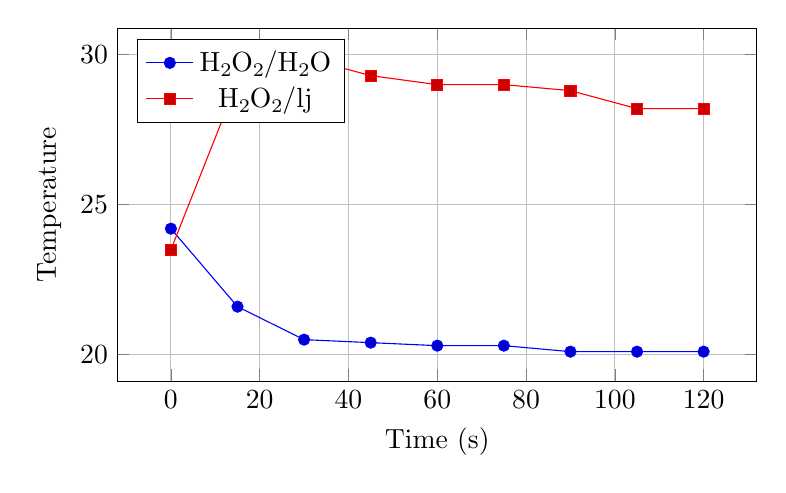
\begin{tikzpicture}
        \begin{axis}[
            xlabel={Time (s)},
            ylabel={Temperature},
            legend pos=north west,
            grid=major,
            width=0.8\textwidth,
            height=0.5\textwidth
        ]
        \addplot coordinates {(0,24.2) (15,21.6) (30,20.5) (45,20.4) (60,20.3) (75,20.3) (90,20.1) (105,20.1) (120,20.1)};
        \addlegendentry{\ch{H2O2}/\ch{H2O}}

        \addplot coordinates {(0,23.5) (15,29.1) (30,29.9) (45,29.3) (60,29) (75,29) (90,28.8) (105,28.2) (120,28.2)};
        \addlegendentry{\ch{H2O2}/lj}
        \end{axis}
    \end{tikzpicture}
    \caption{Graph of Measurements over Time for Procedure A and Procedure B}
    \label{fig:measurements}
\end{figure}

\subsection*{Procedure B}
\begin{table}[h]
    \centering
    \begin{tabular}{cccccccccc}
        \toprule
        Time (s) & 0 & 15 & 30 & 45 & 60 & 75 & 90 & 105 & 120 \\ 
         \midrule
         \ch{H2O2}/boiled lj & 22 & 20.5 & 20.1 & 20.1 & 20 & 20.2 & 20.2 & 20.1 & 20.2 \\ 
         \ch{H2O2}/acid lj & 22 & 21.5 & 21.5 & 21 & 21 & 21 & 21.1 & 21 & 20.9 \\ 
         \ch{H2O2}/base lj & 22 & 21.2 & 21.2 & 21.3 & 21.2 & 21.5 & 21.6 & 21.8 & 21.9 \\ 
         \ch{H2O2}/salt lj & 23 & 23.2 & 24.5 & 26.9 & 28.9 & 31 & 31.5 & 31.9 & 31.7 \\ 
         Boiled \ch{H2O2}/lj & 23 & 31 & 38 & 41 & 41 & 41 & 39 & 38 & 37.5 \\ 
         \bottomrule
    \end{tabular}
    \caption{Table of Measurements over Time for Procedure B}
    \label{tab:measurements_b}
\end{table}
\begin{figure}[h]
    \centering
    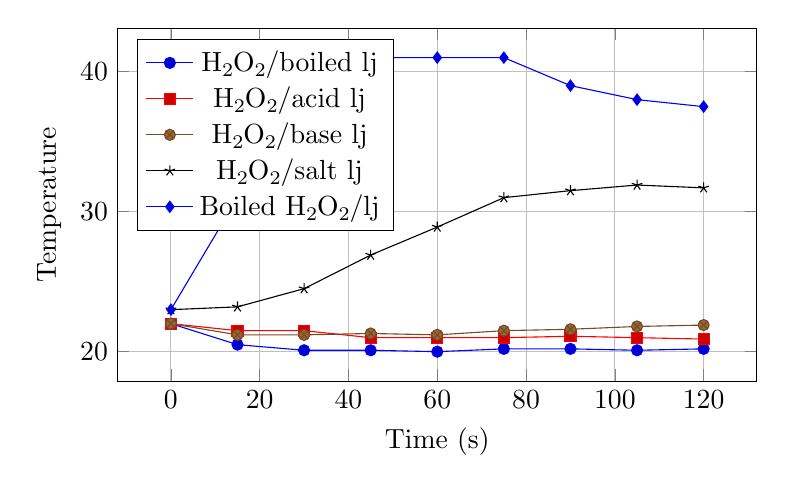
\begin{tikzpicture}
        \begin{axis}[
            xlabel={Time (s)},
            ylabel={Temperature},
            legend pos=north west,
            grid=major,
            width=0.8\textwidth,
            height=0.5\textwidth
        ]
        \addplot coordinates {(0,22) (15,20.5) (30,20.1) (45,20.1) (60,20) (75,20.2) (90,20.2) (105,20.1) (120,20.2)};
        \addlegendentry{\ch{H2O2}/boiled lj}

        \addplot coordinates {(0,22) (15,21.5) (30,21.5) (45,21) (60,21) (75,21) (90,21.1) (105,21) (120,20.9)};
        \addlegendentry{\ch{H2O2}/acid lj}

        \addplot coordinates {(0,22) (15,21.2) (30,21.2) (45,21.3) (60,21.2) (75,21.5) (90,21.6) (105,21.8) (120,21.9)};
        \addlegendentry{\ch{H2O2}/base lj}

        \addplot coordinates {(0,23) (15,23.2) (30,24.5) (45,26.9) (60,28.9) (75,31) (90,31.5) (105,31.9) (120,31.7)};
        \addlegendentry{\ch{H2O2}/salt lj}

        \addplot coordinates {(0,23) (15,31) (30,38) (45,41) (60,41) (75,41) (90,39) (105,38) (120,37.5)};
        \addlegendentry{Boiled \ch{H2O2}/lj}
        \end{axis}
    \end{tikzpicture}
    \caption{Graph of Measurements over Time for Procedure B}
    \label{fig:measurements_b}
\end{figure}


\subsection*{Procedure C}
\begin{table}[h]
    \centering
    \begin{tabular}{cccccccccc}
        \toprule
        Time (s) & 0 & 15 & 30 & 45 & 60 & 75 & 90 & 105 & 120 \\ 
        \midrule
        1.5\% \ch{H2O2} & 22 & 26.1 & 26.9 & 28.9 & 26.5 & 26.2 & 26.2 & 26.1 & 26 \\ 
        3\% \ch{H2O2} & 23 & 29.1 & 30 & 29.9 & 29.1 & 29 & 28.9 & 28.5 & 28.2 \\ 
        6\% \ch{H2O2} & 23 & 34 & 37 & 36.5 & 36 & 35.1 & 34.9 & 34.1 & 33.9 \\ 
        10\% \ch{H2O2} & 23 & 38 & 43 & 42 & 41 & 40 & 39 & 38 & 37.5 \\ 
        \bottomrule
    \end{tabular}
    \caption{Table of Measurements over Time for Procedure C}
    \label{tab:measurements_c}
\end{table}
\begin{figure}[h]
    \centering
    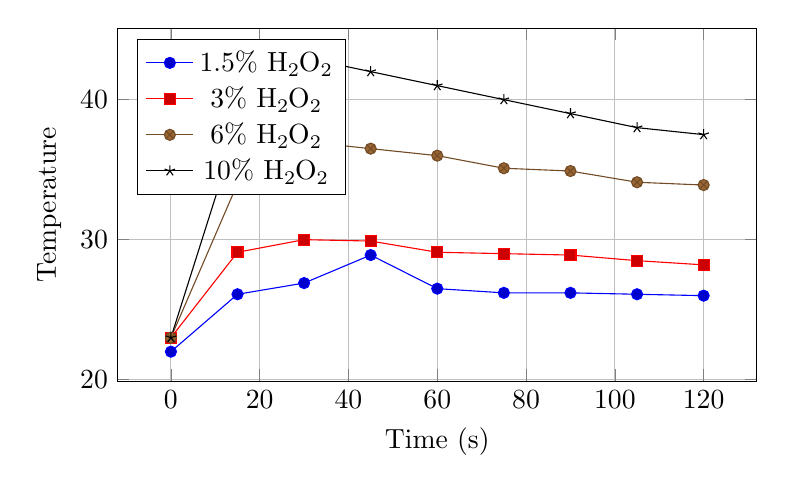
\begin{tikzpicture}
        \begin{axis}[
            xlabel={Time (s)},
            ylabel={Temperature},
            legend pos=north west,
            grid=major,
            width=0.8\textwidth,
            height=0.5\textwidth
        ]
        \addplot coordinates {(0,22) (15,26.1) (30,26.9) (45,28.9) (60,26.5) (75,26.2) (90,26.2) (105,26.1) (120,26)};
        \addlegendentry{1.5\% \ch{H2O2}}

        \addplot coordinates {(0,23) (15,29.1) (30,30) (45,29.9) (60,29.1) (75,29) (90,28.9) (105,28.5) (120,28.2)};
        \addlegendentry{3\% \ch{H2O2}}

        \addplot coordinates {(0,23) (15,34) (30,37) (45,36.5) (60,36) (75,35.1) (90,34.9) (105,34.1) (120,33.9)};
        \addlegendentry{6\% \ch{H2O2}}

        \addplot coordinates {(0,23) (15,38) (30,43) (45,42) (60,41) (75,40) (90,39) (105,38) (120,37.5)};
        \addlegendentry{10\% \ch{H2O2}}
        \end{axis}
    \end{tikzpicture}
    \caption{Graph of Measurements over Time for Procedure C}
    \label{fig:measurements_c}
\end{figure}
























\section*{Data Analysis}

\subsection*{Question 2}
\begin{enumAlph}
    \item 
\end{enumAlph}

\end{document}



\section*{Data Analysis}

\subsection*{Question 2}
\begin{enumAlph}
    \item 
\end{enumAlph}

\end{document}